\chapter{Introduction}

\section{The Active Galactic Nuclei: Quasar vs. Radio Accretion Modes}
Active galaxies constitute a distinctive class characterized by an intensely energetic source at their center, known as an Active Galactic Nucleus (AGN). Since the first observation of an active galaxy in the early 1900s, numerous studies have been conducted on this intriguing category of galaxies. To this day, efforts persist in unraveling the nature and role of active galaxies within the broader context of galactic formation and evolution.

Research in this field has demonstrated that the intense radiation must emanate from a compact region, with a spatial dimension not exceeding 100 parsecs. This estimation was derived from the temporal variability observed in some of these sources \cite{1959ApJ...130...38W}. Additionally, it has been noted that AGNs exhibit luminosity variations of over $50\%$ within timescales ranging from days to years. Such fluctuations can only be explained if a substantial portion of the emission region is randomly connected. These observations strongly imply that the central component of AGNs is likely a Supermassive Black Hole (SMBH), namely a rapidly accreting black hole.

AGN emissions span the entire electromagnetic spectrum, each wavelength band offers insights into specific components and associated phenomena within AGN. 

In addition to the central SMBH \cite{2006ApJ...652..216R} there is a disk of accreting matter onto it, that emits a significant amounts of ultraviolet (UV) radiation. Above this disk, a cloud of relativistic electrons is believed to be there. This cloud reprocess the UV photons emitted from the disk, re-emitting them at X-ray energy levels.
A population of clouds exists in close proximity to the SMBH, that is known as the Broad Line Region
(BLR), because the kinematics of these clouds are significantly affected by the gravitational pull of the SMBH, resulting in broader spectral lines. Beyond the BLR, there exists an outer region surrounding the SMBH known as the Narrow Line Region (NLR). In contrast to the BLR, the NLR is characterized by narrower spectral lines, indicating distinct physical conditions and dynamics. 
 Additionally, surrounding the disk, there's a toroidal-shaped volume composed of a mixture of gas and dust, leading to the partial absorption of central radiation.

The torus is the main component used from the “Unified Model” \cite{1995PASP..107..803U} to explain the existence of different populations of AGN. 
 
\begin{figure}[hbtb]
  \centering
  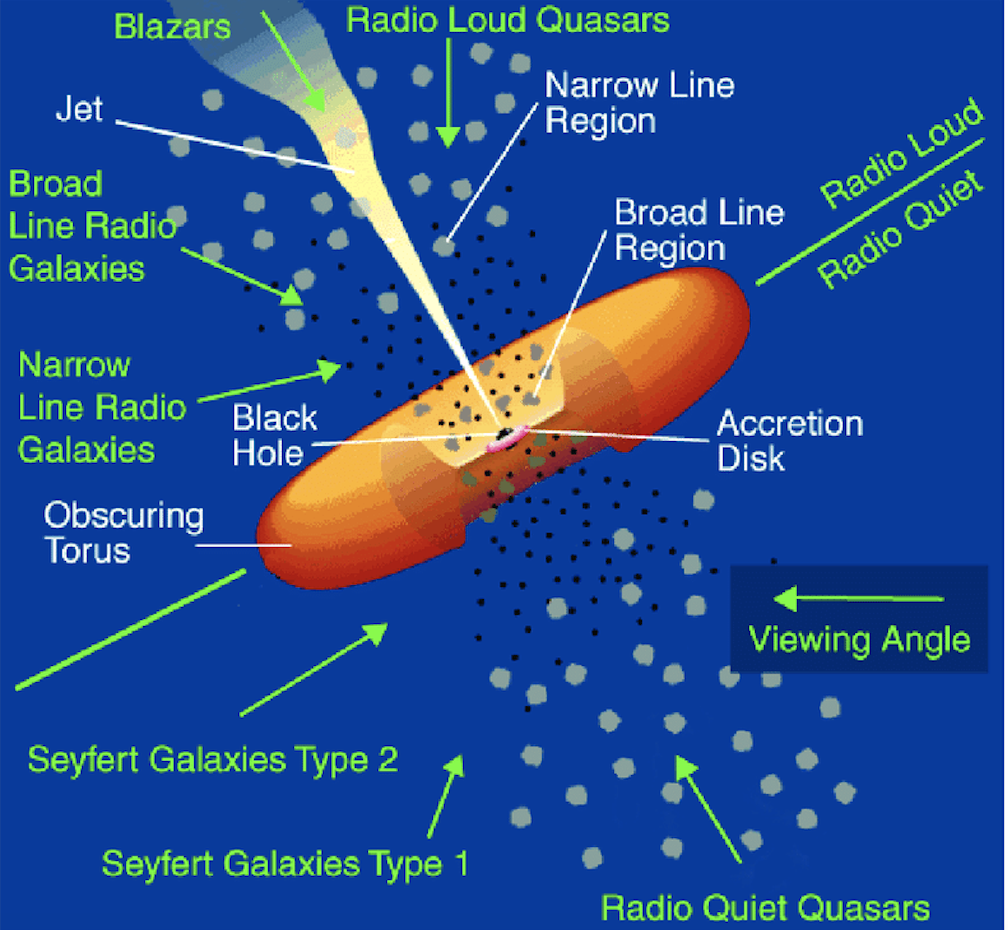
\includegraphics[width=0.5\textwidth]{UnifiedAGNmodel}
  \caption{The Unified AGN model as proposed in \cite{1995PASP..107..803U}}
  \label{2}
\end{figure}


\begin{itemize}
  \item \textbf{Type I:} For these types of AGN, broad emission lines, emitted from the BLR, exhibit a broad component, typically in the range of $\sim 10^{3}$-$10^{4} \text{km s}^{-1}$, along with a narrow emission lines from the NLR. In this configuration, the observer is situated at a small angle relative to the torus axis, allowing the radiation from circumnuclear regions to remain unobscured along the line of sight
  
  \item \textbf{Type II:} In this scenario, the spectrum of the AGN comprises solely narrow emission lines,…, due to the fact that the line of sight… by obscuring the BLR, typically not exceeding $1200 , \text{km s}^{-1}$. In this case, the line of sight intersects the obscuring matter of the torus.
  
\end{itemize}
A visual overview can be found in \autoref{2}.


The energy released during the accretion process of a SMBH plays a significant role in shaping the evolution of the host galaxy \cite{2021A&A...646A.167M}. In this context, the literature often discusses positive and negative feedback mechanisms.
Positive feedback occurring when the AGN feedback promotes stellar formation, while negative feedback involves the suppression of star formation, respectively.

Feedback from SMBH accretion is capable of heating diffuse gas \cite{2005Natur.433..604D} and depositing heavy elements across the extensive surrounding environment \cite{2000ApJ...539L..13G}, with effects observed at scales exceeding kpc scales. 
These models are also capable of halting star formation and consequently depositing metals into the surrounding environment, as suggested in \cite{2000ApJ...539L..13G}.


Two distinct AGN feedback mechanisms have been proposed, each associated with different rates of mass accretion onto the SMBH (Fabian, 2012; Harrison, 2017).
\begin{itemize}
	\item \textbf{QSO's Radiative Feedback :} This feedback mode, often referred as quasar mode, consists in a high accretion 		rate of the SMBH via an optically-thick and geometrically-thin disk, and most of the energy is released in form of radiation.
	\item \textbf{QSO's Radio Feedback :} In this scenario, the SMBH accretion of hotter gas happens with a low rate in a optically-thin and geometrically-thick disk configuration, releasing energy in form of relativistic particles such as Radio Jets.
\end{itemize}



\section{The Brightest Cluster Galaxies }
The Hierarchical model stands as a cornerstone in our understanding of cosmic structure formation, delineating the principal pathways through which galaxies growth their stellar and gas mass assimilating matter from their surroundings.

One of the most extreme examples in this context involves the study of Brightest Cluster Galaxies (BCGs), a unique class of galaxies, situated at the center and typically standing out as the most luminous and massive objects within the entire cluster.( e.g. \cite{2015MNRAS.448....2W} ).

Considering their environment, observational studies, such as \cite{2020MNRAS.498.2719T}, have indicated that the evolution of BCGs differs from the normal galactic path. The prevailing model for cosmic structure formation ( i.e. the Cold Dark Matter Model ) suggests that the mass assembly of BCGs is primarily influenced by dry mergers \cite{2007MNRAS.375....2D, 2019ApJ...881..150C}.

Mainly found to be Elliptical galaxies, BCGs seems to not be drawn from the same luminosity profile as normal elliptic objects outside the cluster environment, and in general has been proven to differ also from generic Bright galaxies.
 ( i.e. \cite{1977ApJ...212..311T}) 
  
Due to their distinct evolutionary histories, the primary mechanism driving the mass growth of galaxies is associated with cooling flows within lower mass halos at high redshifts \cite{2006ApJ...652..216R}.
However, at low redshifts, this phenomenon diminishes, primarily due to increased Active Galactic Nuclei ( AGN ) activity accreting mass into their typically hosted SMBH .
 
As presented before regarding AGN feedback, also BCGs are interested by both of the Quasi Stellar Object modes, resulting in Optical AGN, and Radio Loud Emission such as Radio Jets( e.g. \cite{2007MNRAS.379..867V} ).

These relativistic jets of radio emission are also recognized as one of the main explanation of the so called "Cooling flow problem". The unique relaxed and virialized environment defining the cluster often has cooling time-scales much shorter than Hubble time, that following to the absence of a heating source would lead to the presence of a cooling flow.

However observational studies found that temperature of cluster cores fails to fall below $\sim 30\%$ at large radii resulting in an amount of cooling gas corresponding only to the $\sim 10\%$ expected from the existent cooling flow model. \cite{David_2001}

\newpage
\section{The Aim of this thesis}
In this context, the main scientific question driving this work is to understand \textbf{whether the different evolution of BCGs, along with their "special" environment, affects the accretion of SMBHs in their centers compared to other types of galaxies in the local universe}.

In particular, this study will present a comparative analysis between two representative samples of BCGs and Non-BCGs to highlight the substantial differences that the cluster environment induces in SMBH accretion.


To address this particular inquiry, I conducted an analysis on a BCG sample compiled from the Sloan Digital Sky Survey Data Release 7 (SDSS DR7), as outlined in \cite{2009ApJS..182..543A}, and the C4 BCGs catalogue created by \cite{2007MNRAS.379..867V}. For this specific BCG sample, I utilized the optical line fluxes ($H\alpha$, [OIII], $H\beta$, [NII], and [SII] doublets) provided by the MPA-JHU team to establish a comprehensive understanding of optical AGN presence through the [NII]- and [SII]- BPT diagnostic diagrams. Furthermore, through cross-matching these aforementioned catalogs with datasets derived from NVSS and FIRST radio surveys, as outlined in \cite{2005MNRAS.362....9B}, I identified BCGs displaying radio loud emission, indicative of the existence of radio jets.

These analyses, including data description in subsection 2.1 "Data description" and data analysis in subsection 2.2 "Data analysis," will be comprehensively presented in the "Methods" chapter. 

Following the "Methods" chapter, the subsequent section will delve into the third chapter, concentrating on the disclosure of the acquired outcomes.

